\documentclass[a4paper,12pt]{article}
\usepackage[margin=0.8cm]{geometry}
\usepackage{graphicx}
\usepackage{wasysym}
\usepackage{amsmath,amssymb}
\usepackage{textcomp}
\usepackage{multicol}
\parindent=0pt
\usepackage{fancyhdr}
% day   bible           cheatsheet
% 1     light           light
% 2     firmament       physical constants
% 3a    earth|sea       greek
% 3b    plants          
% 4     sun|moom|stars  relativity
% 5     sea creatures   maths
% 6a    land creatures  linux
% 6b    humanity        vim
% 7     rest            python
%
%
% Maxwells
% Greek alphabet
% maths - trig l'hopital modeling stats
% linux cheatsheet 
% latex cheatsheet
%
%
%
%
%\pagestyle{fancy}
%\rfoot{v1.2}
\newcommand{\sinc}{{\rm sinc}}
\setlength{\columnsep}{20pt}
\begin{document}
\begin{multicols}{2}
In the beginning, there was nothing, which exploded.
\vfill
On the first day, \emph{Maxwell} said..
\[
\begin{array}{rcl}
\nabla \cdot \textbf{E} &=& \frac{\rho}{e_0}\\
\nabla \cdot \textbf{B} &=& 0 \\ 
\nabla \times \textbf{E} &=& -\frac{\partial \textbf{B}}{\partial t}\\
\nabla \times \textbf{B} &=& \mu_0 \textbf{J} + \mu_0\epsilon_0 \frac{\partial
\textbf{E}}{\partial t}\\ 
\nabla &=& \frac{\partial}{\partial x}\textbf{x} +\frac{\partial} {\partial y}
\textbf{y}+\frac{\partial}{\partial z}\textbf{z}\\
\end{array}
\]
in other words $\ldots$

\[
\begin{array}{rcl}
\oiint_{\partial V}\textbf{E} \cdot d\textbf{A} &=& \frac{Q_f(V)}{\epsilon_0}\\
\oiint_{\partial V}\textbf{B} \cdot d\textbf{A} &=& 0\\
\oint_{\partial S}\textbf{E} \cdot d\textbf{l} &=& -\frac{\partial
\Phi_{B,S}}{\partial t}\\ 
\oint_{\partial S}\textbf{B} \cdot d\textbf{l} &=& \mu_0I_S + \mu_0 \epsilon_0
\frac{ \partial \Phi_{E,S}}{\partial t}\\

\end{array}
\]
and then there was light.

\vfill

On the second day, physicists said...
\[
\begin{array}{rcll}
\pi &=& 3.141593 &\\
e &=& 2.718282 &\\
c &=& 299 792 458 & m\cdot^{-1}\\
h &=& 6.626 \times 10^{-34} & J\cdot s\\
\mu_0 &=& 4\pi \times 10^{-7}&N\cdot A^{-2}\\
\epsilon_0 = \frac{1}{\mu_0 c^2}&=& 8.854 \times 10^{-12}& F\cdot m^{-1}\\
q_e &=& 1.602 \times 10^{-19} & C\\
\end{array}
\]
and there was a firmament betweeen the heavens and the earth.
\vfill

On the third day the greeks made significant contributions to language and
mathematics including, their alphabet:
\begin{center}
\begin{tabular}{cclccl}
$\alpha $&$ A $& alpha&$\nu $&$ N $& nu\\
$\beta $&$ B $& beta&$\xi$&$\Xi$& xi\\
$\gamma $&$ \Gamma $& gamma&$o $&$ O $& omicron\\
$\delta $&$ \Delta $& delta&$\pi $&$ \Pi $& pi\\
$\epsilon $&$ E $& epsilon&$\rho $&$ P $& rho\\
$\zeta $&$ Z $& zeta&$\sigma $&$ \Sigma $& sigma\\
$\eta $&$ H $& eta&$\tau $&$ T $& tau\\
$\theta $&$ \Theta $& theta&$\upsilon $&$ \Upsilon $&upsilon\\
$\iota $&$ I $& iota&$\phi $&$ \Phi $&phi\\
$\kappa $&$ K $& kappa&$\chi $&$ X $& chi\\
$\lambda $&$ \Lambda $& lambda&$\psi $&$ \Psi $& psi\\
$\mu $&$ M $& mu&$\omega $&$ \Omega $& omega\\
\end{tabular}
\vfill
\begin{tabular}{lllll}
n&& $10^n$&&$10^{-n}$\\
3& k & kilo & m & milli\\
6& M & mega & $\mu$ & micro\\
9& G & giga & n & nano\\
12& T & tera & p & pico\\
15& P & peta & f & femto\\
18& E & exa & a & atto
\end{tabular}
\end{center}
\vfill
\columnbreak
And trigonometry.
\[
\begin{array}{rcl}
\sin(x\pm y)&= &\sin x\cos y \pm \cos x \sin y\\ 
\cos(x\pm y)&= &\cos x \cos y \mp \sin x \sin y\\
\tan(\alpha \pm \beta)&=&\dfrac{\tan\alpha\pm\beta}{1\mp\tan\alpha\tan\beta}\\
\sin^2\theta = \cos^2\theta&=& \dfrac{1-\cos 2\theta}{2}\\
\sinc x&=&\dfrac{\sin\pi x}{\pi} \mbox{ \ normalized}\\
\end{array}
\]
\vfill

On the fourth day \emph{Einstein} noticed that
\[ E=mc^2 \]
and there were stars and atoms were produced to build the planets and moons.
\vfill
On the fifth day many mathematicians did make the earth teem with equations and
their minds were filled with models of the world.
\vfill
\emph{Bayes} did say \ \ 
\[
\begin{array}{ll}
p(B|A) = \dfrac{p(A|B)p(B)}{p(A)}&p(A)=\mbox{prior prob}\\
&p(B|A)=\mbox{prob B given A}\\
\end{array}
\]
\vfill
The statisticians defined.. $E[X]=\mu_X$
\[
\begin{array}{rcl}
var[X]=\sigma_X^2&=&\frac{1}{n-1}\sum (X-\mu^2)=E[X^2]-(E[X])^2\\
cov[XY]&=&\frac{1}{n-1}\sum(X-\mu_X)(Y-\mu_Y)\\
cov[XY]&=&E[XY]-E[X]E[Y]\\
\end{array}
\]
\vfill
\emph{L'Hopital} declared that...

\[\mathop {\lim }\limits_{x \to c} \frac{{f\left( x \right)}}{{g\left( x
\right)}} = \mathop {\lim }\limits_{x \to c} \frac{{f'\left( x
\right)}}{{g'\left( x \right)}}\]


\vfill
\emph{Newton} did  also observe that \textbf{physical systems} could be
modelled using a calculus.

\[
\begin{array}{cccl}
v = Ri&i = C\dfrac{\partial v}{\partial t}&v = L\dfrac{\partial i}{\partial
t}\\

P = i^2R & E_C = \dfrac{Cv^2}{2} & E_L = \dfrac{Li^2}{2}& E = \mbox{energy}\\

\mbox{damper}&\mbox{spring}&\mbox{mass}&f_v = \mbox{friction}\\
f = f_v v   & v = \dfrac{1}{K}\frac{\partial f}{\partial t}&f =
M\dfrac{\partial v}{\partial t}&v = \mbox{velocity}\\ f = f_v\dfrac{\partial
x}{\partial t}    &   f=Kx    & f = M \dfrac{\partial^2 x}{\partial t^2}&f =
\mbox{force}
\end{array}
\]

\columnbreak

On the sixth day, \emph{Stallman} did declare that sofware should be free. Free as in
speech. And \emph{Linus} did decree...

\begin{tabular}{ll}
%\texttt{w}& display who is online\\
\texttt{uname -a}& kernel config\\
\texttt{lsb\_release -rcs}& release version\\
\texttt{grep patt files}& find pattern in files\\
\texttt{command \&}& run command in bg\\
\texttt{fg n}& bring n to fg\\
\texttt{fg}& bring most recent to fg\\
\end{tabular}

\vfill
%But a GNOME did appear..
%
%begin{tabular}{ll}
%texttt{alt+tab}&switch windows\\
%texttt{alt+esc}&in reverse order\\
%texttt{ctrl+PgUp}&previous terminal tab\\
%texttt{SUPER+4}&change rating to 4 in Amarok\\
%\end{tabular}
%\vfill
%\bigskip
\emph{Google} did declare that things could be done better.

\bigskip

\begin{tabular}{ll}
&\texttt{GMAIL}\\
\texttt{o}&expand/collapse msg/convo\\
\texttt{c|u}&compose \textbar{} escape\\
\texttt{j|k}&older \textbar{} newer conversation\\
\texttt{n|p}&next \textbar{} previous message\\
\texttt{x}&select conversation\\
\texttt{y}&archive \textbar{} unstar \textbar{} remove label\\
\texttt{e|m}&archive \textbar{} mute conversation\\
\texttt{+|-}&important \textbar{} unimportant\\
\texttt{s}&star msg or convo\\ 
\texttt{!|\#}&report spam \textbar{} delete\\ 
\texttt{r|a}&reply \textbar{} all\\ 
\texttt{f}&forward\\ 
\texttt{ctrl+s}&save\\
\texttt{/}&search\\ 
\texttt{gi}&goto inbox\\
\texttt{g a|s}&goto all mail \textbar{} starred\\ 
\texttt{g c|d}&goto contacts \textbar{} drafts\\ 
&\\
&\texttt{CALENDAR}\\
\texttt{k|p j|n}&previous next\\
\texttt{t}&jump to today\\
\texttt{q|c}&quick add \textbar{} new event\\
\texttt{d|w}&day \textbar{} week view\\
\texttt{m|a}&month \textbar{} agenda view\\
\texttt{alt+s}&save event\\
\\
%&\texttt{CHROME}\\
%\texttt{ctrl}&\emph{precedes all following cmds}\\
%\texttt{n}&goto tab n\\
%\texttt{w}&close tab/popup\\
%\texttt{9}&last tab\\
%\texttt{PgDown}&next tab\\
%\texttt{PgUp}&prev tab\\
%\texttt{shift+t}&reopen closed tab\\
%\texttt{l}&highlight url\\
%\texttt{f}&open find bar\\
&\texttt{VIMIUM}\\
&\emph{remember cmd repetition etc.}\\
\texttt{d}&down half a page\\
\texttt{f|F}&open link \textbar{} in new tab\\
\texttt{r}&reload\\
\texttt{zi|zo|z0}&zoom\\
\texttt{yy}&copy url\\
\texttt{gf}&goto next frame\\
\texttt{/|n|N}&find \textbar{} next \textbar{} prev\\
\texttt{H|L}&back \textbar{} forward\\
\texttt{J|K}&tab left \textbar{} right\\
\texttt{t|x|X}&create \textbar{} close \textbar{} restore tab\\
\texttt{[[ | ]]}&prev \textbar{} next\\
\texttt{gi}&go to first (or nth) text input\\
\end{tabular}
\vfill
\columnbreak
The community declared that Vi should be iMproved, and Vi was improved to
create ViM, the nerdiest of the text editors (except for emacs).
\bigskip

\begin{tabular}{ll}
&\texttt{MOVING}\\
&\emph{remember to prepend repetitions}\\
%\texttt{w|W}& next word \textbar{} spaces\\
%\texttt{b|B}& back word \textbar{} spaces\\
\texttt{e|E}& end of word \textbar{} spaces\\
\texttt{z[b|t|z]}& scroll\\
\texttt{fx|Fx}& move forward \textbar{} backward to x\\
\texttt{(|)}& move to previous \textbar{} next sentence\\
\texttt{nG}& go to line n\\
\texttt{\^{}}& first char of line\\
\texttt{0|\$}& BOL \textbar{} EOL\\
\texttt{gg|G}&BOF \textbar{} EOF\\
\texttt{\`{}.}& line last edited\\
\texttt{gd}& definition of variable\\
\texttt{\#|*}& previous \textbar{} next occurance of word\\
\texttt{\%}& matching brace\\
\\
&\texttt{EDITING}\\
&\emph{remember to use movement commands}\\
%\texttt{i|I}& insert \textbar{} beginning of line\\
%\texttt{a|A}& append \textbar{} end of line\\
\texttt{r|R}& replace \textbar{} many chars\\
\texttt{J}& join line below to current\\
\texttt{c|C|cc}& replace \textbar{} to EOL \textbar{} linewise\\
\texttt{y|Y|yy}& yank \textbar{} to EOL \textbar{} linewise\\
\texttt{d|D|dd}& delete \textbar{} to EOL \textbar{} linewise\\
\texttt{p|P}& paste \textbar{} before cursor\\
\texttt{u|U}& undo \textbar{} linewise\\
\texttt{v|V}& start visual \textbar{} linewise\\
\texttt{<|>}& deindent \textbar{} indent\\
\texttt{\~}& switch case\\
\\
&\texttt{SPELL\ \ \ :set spell}\\
\texttt{[|]s}&prev \textbar{} next\\
\texttt{zg}&add to dictionary\\
\texttt{zug}&undo addition to dictionary\\
\texttt{z=}&view spelling suggestions\\
\end{tabular}

\vfill

\begin{tabular}{ll}
&\texttt{COMMANDS}\\
&\emph{entered after }\texttt{ :}\\
\texttt{/ptn}& search for pattern\\
\texttt{?ptn}& search backward\\
\texttt{n|N}& repeat search \textbar{} backwards\\
\texttt{\%s/old/new/g}&replace all old with new\\
\texttt{8,20s/\$/text/}&append text to lines 8-20\\
\texttt{s/\^{}/txt/}&prepend text to current line\\
\texttt{bd}&close buffer\\
\texttt{sp}&open file and split window\\
\texttt{ctrl+ws}&split window\\
\texttt{ctrl+ww}&switch windows\\
\texttt{ctrl+ww}&quit a window\\
\texttt{ctrl+wv}&split vert\\
\end{tabular}

\clearpage
On the seventh day. The machines became aware.
\begin{tabular}{l}
OBTAIN\\
\texttt{lynx -dump url} get text of page\\
\texttt{curl url/apicall}\\
\texttt{wc } word count\\
\\
SCRUB\\
\\
EXPLORE\\
print some random lines\\
\texttt{cat file | sort -R | head -n 10}\\
\texttt{less file} \emph{remember Vim cmds}\\
MODEL\\
\\
INTERPRET\\
\\
\end{tabular}

\begin{tabular}{l}
Python Tricks\\
\texttt{if "str" in string:}\\
\texttt{\ \ \  print "str is in string"}\\
Pretty print a list\\
\texttt{print ",".join(list\_of\_things)}\\
Filtering lists:\\
\texttt{numsUnder4 = filter(lambda x: x < 4,nums)}\\
is equivalent to\\
\texttt{numsUnder4 = [n for n in nums if n < 4]}\\
Generator Expressions are more efficient:\\
\texttt{squaresU10 = (n*n for n in nums if n*n < 10)}\\
Each successive value of squaresU10 can be gotten by calling .next(), or\ldots\\
\texttt{for s in squaresU10:}\\
\texttt{\ \ \  print s}\\
Reducing:\\
\texttt{result = reduce(lambda a,b: a*b, numbers)}\\

\end{tabular}
%TODO command line tools
%http://www.pixelbeat.org/cmdline.html
\vfill
Stand back. I know regular expressions.
% http://www.addedbytes.com/cheat-sheets/regular-expressions-cheat-sheet/
\bigskip
\begin{tabular}{ll}
\texttt{([A-Za-z0-9-]+)}&letters, numbers and hyphens\\
\end{tabular}
\vfill
``All models are wrong, some are useful.'' - George Box
\vfill
\clearpage

\subsection*{EE Stuff}
\begin{tabular}{ll}
Norton&$I_{sc} || R_{oc}$\\

Thevenin&$V_{oc} + R_{sc}$\\

Max power &$R_L = R_{thevenin}$\\

NVA$\rightarrow$KCL$\rightarrow$& $\dfrac{v_{ab}}{R_1} + \dfrac{v_{ac}}{R_2} +
\cdots = 0$\\

MCA$\rightarrow$KVL$\rightarrow$& $R_1i_1 + R_2i_2 + \cdots = 0$\\
\end{tabular}

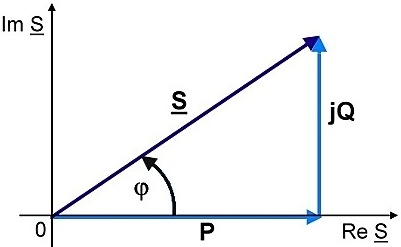
\includegraphics[width=40mm]{ACPower.jpg}
\begin{tabular}{cc}
real \textbar{} reactive & R \textbar{} Q\\
complex  apparent& S \textbar S\textbar\\
power factor & $\cos \psi$\\
$ \jmath \omega L = $&$ Z_L$\\
$\dfrac{-\jmath}{\omega C} = \dfrac{1}{\jmath \omega C} = $&$Z_c$\\
\end{tabular}
\vfill
\[
A_{v/i} = 20 \log_{10}{|A_{v/i}|} dB \hspace{15 mm} A_p = 10 log|A_p| dB
\]
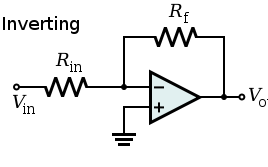
\includegraphics[width=70mm]{inverting-amp.png} 

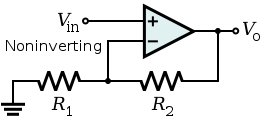
\includegraphics[width=70mm]{noninverting-amp.png} 
\vfill
Differential input is $v_1 - v_2$ Common mode input is $\dfrac{v_1+v_2}{2}$

Amplifier Types: V,I, Transconductance ($G_m=\dfrac{i_o}{v_i}$),
Transresistance ($R_m=\dfrac{v_o}{i_i}$)

Ideal Inputs and Outputs: 
\begin{tabular}{ccc}
i&$R_i=0$&$R_o=\infty$\\
v&$R_i=\infty$&$R_o=0$\\
\end{tabular}
%\subsubsection*{Diode Models}
%\begin{description}
%\item[Constant voltage drop] ideal + $v_{DD} = 0.7$
%\item[Piecewise linear] (ideal + $v_{DD} + r_D$) slope is $\frac{1}{r_D}$
%\item[small signal] slope $=\frac{1}{r_D}$ where $r_d = \frac{n V_T}{I_D}$ and
%$i_D = \frac{v_d}{r_d}$ \end{description}
\subsubsection*{2104 Odds and Ends}

\begin{tabular}{cl}
half wave&$\tau= RC$\\
$V_r = V_p \dfrac{T}{\tau} = V_p\dfrac{1}{f\tau }$&$v_r$ is v drop\\
full wave&$T$ is discharge time\\
$V_r = \dfrac{V_p}{2f\tau }$&f \mbox{ is the supply freq}\\
new freq is&$2f$\\
\end{tabular}
% \mbox{ new freq}\]

\vfill

\[
\begin{array}{ccc}
Line    &   Load    &   Voltage\\
\dfrac{\Delta V_O}{ \Delta V_s} &\dfrac{\Delta V_O }{\Delta I_L }&\dfrac{V_{NL}
- V_{FL}}{V_{NL}}\\

\mbox{ s = source} & \mbox{O = output}&\Delta \mbox{ = percentage}\\
\end{array}
\]
\vfill
BJT... \emph{current flows in direction of arrow}
\[ 
\begin{array}{cc}
I_E = I_C + I_B&\mbox{pnp }=  E \rightarrow B\\
\alpha = \frac{I_C}{I_E}& \beta = \frac{I_C}{I_B}\\
\alpha = \dfrac{\beta}{\beta + 1}&\\
\end{array}
\]
\vfill
Hybrid $\pi$ model. Add resistor $r_0$ in parallel to $I$ source for Early effect.
\[ 
\begin{array}{cc}
v_\pi = v_{BE}&r_\pi = r_{BE}\\
i_{C} = \beta i_b = g_m v_\pi&\\
\end{array}
\]
T Model has 
\[i_c = g_m v_{be} = \alpha i_e \mbox{ and }v_{be} = i_e r_e\]
Relating the T model and hybrid $\pi$ model.
\[ r_\pi = (\beta + 1 )r_e\]
MOSFET \ \ \ \ \emph{ where} $\beta$ always = $\infty$
\medskip

When $v_{GS} \ge V_t$ the channel is conductive. 
\smallskip

$L$ is length between $S$ and $D$ doped (0.1-3$\mu$m). 
\smallskip

$W$ is width of device (0.2-100$\mu$m).
\smallskip

$k^\prime_n$ is the transconductance $\left(\dfrac{A}{V^2}\right)$.

NMOS has n gates and P substrate. PMOS has p gates and N substrate (usually an
N well in P substrate). We ignore the voltage of the body (B).

Polarity of voltage determines which side is source or drain. Drain is
\emph{always positive relative to source in n-channel MOSFET}. Arrow is at
source end. Points to source in n-channel, away in p-channel.

Triode region is where $v_{DS} \le v_{GS} - V_t$

\subsubsection*{2104 Formulae}
BJT Equations
\[
\begin{array}{cc}
i_c = I_S e^{v_{BE}/V_T}    & g_m = \dfrac{I_C}{V_T}\\
r_e = \dfrac{V_T}{I_E}       &r_o = \dfrac{V_A}{I_C}
\end{array}
\]
MOSFET equations
\[ i_D = \frac{1}{2} k_n^\prime \frac{W}{L}(v_{GS} - V_t)^2 = k(v_{GS} -
V_t)^2\]

\[g_m = k_n^\prime \frac{W}{L} (V_{GS} - V_t) = \frac{2i_D}{(V_{GS} - v_t)}\]
JFET equations
\[i_D = I_{DSS} \left(1 - \frac{V_{GS}}{V_P}\right)^2\]
\[g_m = \left(\frac{2I_{DSS}}{|V_p|}\right)\sqrt{\frac{I_D}{I{DSS}}}\]
\subsubsection*{3405 Stuff}
Gain of a feedback amp:
\[ A = \dfrac{x_0}{x_i}=\dfrac{a}{1+a\cdot \beta}\]
\columnbreak
\subsubsection*{Signals and Systems}
Unilateral laplace properties \[x \rightarrow x(t) \mbox{ and } X \rightarrow X(s)\]

\begin{tabular}{crcll}
linearity& $a_1x_1 + a_2x_2i$&$\leftrightarrow $&$a_1X_1+a_2X_2$&\\
time shift& $x(t-t+0) $&$\leftrightarrow $&$X(s)e^{-t_0s}$ & $t_0 > 0$\\
time scale&$x(at)$&$ \leftrightarrow $&$X\left( \frac{s}{a} \right)$ & $a>0$\\
cplx shif& $e^{-at}x $&$\leftrightarrow $&$X(s+a)$&\\
conv& $x(t)*h(t) $&$\leftrightarrow $&$X(s)H(s)$&\\
\end{tabular}

\[Y(s) = X(s)\left[ \frac{A(s)}{1+A(s) \beta (s)}\right] \]
Some Transforms
\[
\begin{array}{cc}
d{t}&1\\
u(t)&\dfrac{1}{s}\\
t^n e^{\lambda t} u{t}& \dfrac{n!}{(s - \lambda)^{n+1}}\\
e^{-at}\cos{(bt)}u(t)& \dfrac{s+a}{(s+a)^2 + b^2}\\
e^{-at}\sin{(bt)}u(t)& \dfrac{b}{(s+a)^2 + b^2}\\
\end{array}
\]

Differentiation in time
\[
\begin{array}{l}
\frac{\partial^n x(t)}{\partial t^n} \leftrightarrow s^nX(s) - \\
\left(s^{n-1} x(0^-) + s^{n-2}\left[\frac{\partial x(t)}{\partial
t}\right]_{t=0^-}+ \ldots + \left[\frac{\partial^{n-1}x(t)}{\partial t^{n-1}}
\right]_{t=0^-}\right) \end{array}
\]
for example \ldots 
\[\frac{\partial x(t)}{\partial t} \leftrightarrow sX(s) - x(0^-)\]
\[t^nx(t) \leftrightarrow (-1)^n \frac{\partial^nX(s)}{\partial x^n}\]

Integration in time
\[
\int^t_{0} x(\tau) d\tau \leftrightarrow \frac{1}{s}X(s) +  x(0^-)
\]
\begin{tabular}{cccc}
IVT&$x(0^+)$&=&$\lim_{s \to \infty} sX(s)$\\
FVT&$\lim_{t\to \infty} x(t)$&=&$\lim_{s\to \infty} sX(s)$
\end{tabular}

\clearpage
\subsection*{Communications}
The OSI model

\begin{tabular}{cll}
&layer&examples\\
7&application&http nfs ftp\\
6&presentation&MIME SSL\\
5&session&\\
4&transport&TCP UDP\\
3&network&IPv4 ICMP\\
2&data link control&PPP DHCP\\
1&physical&802.11 802.3\\
\end{tabular}

Elements of a Digital System

\begin{tabular}{cc}
information&\\
&(message signal)\\
source encodeer&\\
&(source codeword)\\
channel encoder&\\
&(channel codeword)\\
digital modulator&\\
&(waveform)\\
channel&\\
\end{tabular}

\subsubsection*{Shannon's information capacity theorem}

Constraints (power, bandwidth, cost)

Reliability is measured by Bit Error Rate (BER)
\[
C = B \log_2 (1+SNR) \mbox{ \ \ bits per second}
\]
\begin{description}
\item[C] information capacity
\item[B] channel bandwidth
\item[R] signaling rate
\item[SNR] signal / noise ratio
\item[W] message bandwidth
\end{description}
\[
\eta = \frac{R}{C} \mbox{ \ \ measure of system efficiency}
\]

\subsubsection*{Continuous Wave Modulation}
\textbf{AM}
\begin{align*}
c(t) &=A_c \cos (2\pi f_ct)& \mbox{ carrier}\\
m(t) &  &\mbox{bband sig}\\
s(t) &=A_c \cos \left[1+K_am(t)\right] \cos(2\pi f_ct) &\mbox{modulated}\\
\end{align*}

Envelope of s(t) has the same shape as m(t) for $|K_a m(t)| < 1$ and $f_c >> W$

Fourier Transfom:
\[S(f) = 1/2 A_c [\delta(f-f_c)+\delta(f+f_c)]\]
\[+ 1/2K_aA_c[M(f-f_c)+M(f+fc)]\]


\begin{description}
\item[] Linear modulation techniques
\item[DSB-SC] $s_l(t) = m(t) , s_Q(t) = 0$
\item[SSB-LSB] $s_l(t) = 1/2 m(t) , s_Q(t) = 1/2\hat m(t)$
\item[SSB-USB]$s_l(t) = 1/2 m(t) , s_Q(t) = - 1/2\hat m(t)$
\item[VSB] vestigial sideband
\item[vestige of lsb]$s_l(t) = 1/2 m(t) , s_Q(t) =  1/2m'(t)$
\item[vestige of usb]$s_l(t) = 1/2 m(t) , s_Q(t) = - 1/2m'(t)$
\item[$m'$] output of filter of freq response of $H_Q(f)$
\item[$\hat m$] hilbert transform of $m(t)$
\end{description}

\textbf{Double Sideband - Suppressed Carrier (DSB-SC)}
\[s(t) = A_c m(t) cos(2\pi f_c t)\]
\[S(f) = \frac{A_c}{2}[M(f-f_c)+M(f+f_c)]\]
Required bandwidth = 2W
Spectrum  /\textbackslash \_\_ \textbar \_\_/\textbackslash

\[v_0(t) = 1/2 A_cA'_c \cos \phi m(t)\]
To be proportional $\phi$ is constant, using `quadrature null effect' of a
coherent detector we can send two independant message signals over the same
channel (90\textdegree out of phase).

\textbf{Single Sideband modulation}
Use a filter to remove other sideband, the message spectrum must have an
\emph{energy gap} centred at the origin.


\begin{description}
\item[Angle Modulation - PM and FM] Angle modulated signal: $s(t) = A_c
cos[\theta_i(t)]$ where $\theta_t=$ is the angle of a modulated carrier.
\item[modulating process]
\item[FM] integrator then phase modulator
\item[PM] differentiator then frequency modulator
\item Zero crossings of PM/FM are not regular. 
\item FM and PM signals have constant envelope.
\item we only discuss FM
\item[PM] $\theta_i(t) = t\pi f_ct + k_p m(t)$
\item[$k_p$] phase sensitivity constant
\item[thus] $s(t) = A_c cos[2\pi f_ct + k_pm(t)]$
\item[FM] $f_i(t) = f_c + k_f m(t)=f_c+\Delta f \cos (2\pi f_m t)$
\item[$\Delta f = k_f A_m$] frequency deviation
\item[$k_f$] frequency sensitivity constant
\item[thus] $s(t) = A_c cos[2\pi f_ct + 2\pi k_f\int^t_0m(\tau)d\tau]$
\item[$\beta = \Delta f / f_m$] modulation index
\item[narrowband FM] $\beta <<1$ radian, not ideal
\item[wideband FM] $\beta >>1$ radian
\item[power] envelope of FM is constant and avg power is $P=1/2 A_c^2$
\item FM signals have $\infty$ side freqs $\rightarrow \infty$ BW
\item[in practice] for large $\beta$ BW is slightly greater than $2\Delta f$
\item[Carson's rule] for BW of FM $B_T \approx 2\Delta f + 2f_m = 2\Delta
f(1+1/\beta)$

\item[Nonlinearity] of FM: FM is not afffected by distortion, but is
\emph{extremely sensitive} to phase non-linearity.

\item[AWGN] additive white gaussian noise
\item[BP filter] in reciever
\item[$N_0/2$] power spectral density of noise $w(t)$ for pos and neg freqs 
\item[$N_0$] avg noise power per unit bandwidth measured at front end of
reciever 
\end{description}

%\subsubsection*{Pulse Modulation}
%\begin{description}

%\end{description}


\clearpage
\subsection*{Financial Markets}
Types of markets: \emph{equity/stock, bond, money/credit, commodity, physical
asset, FOREX, derivatives}.

Risk averse preferences under uncertainty == MU falling as wealth increases...
risk averse/neutral/loving leads to indifference curves.

An Edgworth box traces the outline of all possible allocations of 2 assets. An
allocation of the endowment that improves the welfare of a consumer without
reducing the welfare of another is a Pareto-improving allocation. Since
consumers can refuse to trade the only outcomes from trade are pareto
improving. 

\begin{description}
\item[risk] probabilities known
\item[uncertainty] probabilities unknown
\end{description}
The \emph{expected utility hypothesis} implies that probs are applied to each
state and that the decision maker maximises the expected utility...
\[E[u(W)]=U(W_1,...W_l)=\pi_1u(W_1)+...\pi_lu(W_l)\]
\subsubsection*{Risk aversion (RA)}
\[
\begin{array}{rl}
u''(W) < 0 &\mbox{averse}\\
u''(W) = 0 &\mbox{neutral}\\
u''(W) > 0 &\mbox{loving}\\
-W\frac{u''(W)}{u'(W)} &\mbox{index of rel RA}\\
\frac{-u''(W)}{u'(W)} &\mbox{index of abs RA}\\
\mbox{CRRA }u(W) =  &W^{1-\gamma}/(1-\gamma) \mbox{ if } \gamma \ne 1\\
                    &lnW \mbox{ if } \gamma = 1\\
\mbox{CARA }u(W) =& 1-e^{\phi W} \phi > 0\\
\mbox{quadratic }u(W) =&W - bW^2, b>0\\
\end{array}
\]

\subsubsection*{Portfolio Selection in EUH...}

\begin{tabular}{rl}
&\\
\emph{Some definitions...}&\\
budget constraint& $p_1x_1+..+p_nx_n=A$\\
A &initial wealth\\
$x_j$, $p_j$&holding, price of asset $j$\\
$a_j=p_jx_j/A$& proportion invested in $j$\\
terminal wealth& $W = (1 + r_p)A$\\
$r_p$& is rate of return  \\
$v_j=(1+r_j)p_j$ & payoff of asset $j$\\
$x_0$&holding of risk free asset\\
$v_{kj}$& arrow security pays 1 if\\
&$k=j$ and 0 otherwise\\
$r_0$&risk free asset\\
\end{tabular}
\begin{tabular}{rl}
$var[W]$&$=E[W-E[W]]^2i$\\
        &$E[W^2]-[E[W]]^2$\\
$\mu_j=E[r_j]$&$\mu_P=E[r_P]$\\
$\sigma_{jP}$&$=cov[r_j,r_P]$\\
$\sigma_j=+\sqrt{\sigma_{jj}}$&stdev of $j$\\
$\rho_{ij}=\sigma_{ij}/(\sigma_i\sigma_j)$& correlation coefficient\\
$a_0,a_1,a_2,\ldots,a_n$&portfolio\\
$\mu_P=\sum^n_{j=0}a_j\mu_j$&return of portfolio\\
$\sigma^2_P=\sum^n_{i=0}\sum^n_{j=0}a_ia_j\sigma_{ij}$&var of portfolio\\
$\sigma_{jP}=\sum^n_{i=0}a_i\sigma_{ij}$&covar between$j$ and $P$\\
$s_j=\frac{\mu_j-r_0}{\sigma_j}$& Sharpe ratio\\
&\\
\end{tabular}

An \emph{Arbitrage Portfolio} is where $A = 0$

The \emph{Fundamental Valuation Relationship} is a collection of first order
conditions, one for each asset. In general form: \[E[(1+r_j)H]=1 \mbox{for all
j}\]

H is a random variable specific to the context. It varies across states and
agents, reflecting agents' holdings of portfolios.


\[\mathcal{L}=\pi_1u(W_1)+\pi_2u(W_2)+...+\pi_lu(W_l)+\]
\[\lambda(A-p_0x_0-p_1x_1-p_2x_2-..-p_nx_n)\]
where
\[W_k=v_0x_0+v_{k1}x_1+v_{k2}x_2+...+v_{kn}x_n\]
The fundamental Valuation Relationship for (single period) portfolio allocation
problem is:

\[E[(1+r_j)u'(W)]=\lambda \mbox{ for all } j\]
\[H_k=u'(W_k)/\lambda\]
\subsubsection*{Implications of complete asset markets}
\emph{If} agents agree on probs and asset markets are complete then $H$ becomes
common ($H_k$ may still differ across agents as $u(W)$ differs). We need arrow
securities or to construct portfolios that pay in only one state.

\subsubsection*{Risk Neutrality}
FVR in presence of risk free asset
\[E[(r_j-r_0)u'(W)]=0\]
Risk neutrality $u''(W)=0$ means $u'(W)=c$, substituting these into the FVR we
get $E[r_j]=r_0$ << this is an identity. If it does not hold an investor will
borrow at $r_0$ and invest in an asset with the highest $E[r_j]$

So optimization of portfolios for risk-neutral agents is a moot question.

\subsubsection*{Mean-Variance Model}
Assume $u(W)=W-bW^2$ then
\[E[u(W)]=F(E(W),var[w])\]
using variance defs we get 
\[E[u(W)]=E[W]-b[var[W]+(E[W])^2]\]
variance of the portfolio
\[\sigma^2_P=E[(r_P-\mu_P)^2]\]
FVR in quadratic $u$ case
\[\frac{\mu_j-r_o}{\sigma_{jP}/\sigma{P}}=\frac{\mu_P-r_0}{\sigma_P}\mbox{ for
all } j\]

So $\sigma_{jP}/\sigma_P$ is the increment to risk if we hold a bit more of
$j$.

FVR states that the expected return to any asset ( $\mu_j - r_0$) has to be
proportional to its contribution to overall risk $\sigma_{jP}/\sigma{P}$.

Investor acts to maximize $G(\mu_P,\sigma^2_P)$ the shape of G depends on the
utility function. 

$G=\mu_P-\alpha \sigma^2_P$ is a popular example (if all asset returns are
normally dist and 

$u=1-e^{\phi W}$) then $G$ is equivalent to expected utility maximisation and
$\alpha=\frac{\phi}{2}$. 

\subsubsection*{Intertemporal choice and the equity premium puzzle}

Consideer two periods where  all wealth is consumed at $t+1$.

\begin{tabular}{rl}
$C_t, C_{t+1}$& consumption\\
$W_t, W_t-C_t$& endowments\\
$C_{t+1}=(1+r_{t+1})(W_t-C_t)$& IT budget constriaint\\
$U(C_t,C_{t+1})=$&$u(C_t)+\delta u(C_{t+1})$\\
$\delta$& subjective disc factor\\
$(1/\delta)-1$& rate of time prefs\\
$u'>0$&$u''<0$\\
\end{tabular}

Uncertainty: Recall FVR, if EUH holds:

\[H=\delta\frac{u'(C_{t+1})}{u'(C_t)}\]
\begin{description}
\item[Lifetime portfolio selection] conventional wisdom is to take more risk
when young. Not according to this model.

\item[abandoning the EUH] we can consider a \emph{target wealth} or
\emph{minimizing the risk of loss} model.

\item[The role of human capital] if labour income is risky (risk of redundancy)
then less risk is taken with portfolio. Can argue that young people, secure in
their jobs should invest in equities. Older people have lower humancapital and
should invest in bonds.

\item[The Equity Premium Puzzle] Investors tend to favour low-risk bonds to
their detriment. The value of $\gamma$ needed to justify the premium is around
8.5 whereas most studies in other contexts found $\gamma$ to be less than 3.

\item[risk free rate puzzle] investors transfer too much wealth from the
present to the future for plausible values of $\delta$

\end{description}

What to do... MEASURE HOW PEOPLE BEHAVE \emph{ - David Griffin}

\subsubsection*{The Mean Variance $(\mu,\sigma)$ Approach}
Plane is $\mu_P,\sigma_P)$. Draw triangle between asset 1, asset 2 and V on
vert ($\mu_P$) axis. V is the risk free portfolio. Portfolios can exist inside
triangle and outside triangle if we allow short selling. If there is no risk
free asset we start with two assets, combine them and continue.

\emph{First mutual fund theorem} of portfolio analysis: given $n>2$ portfolios,
there exist two composite assets (mutual funds) such that evry
$(\mu_P,\sigma_P)$ on the efficient frontier can be obtained holding only the
two fuds.

$r_0$ and $r_l$ if it is different are on the vertical axis. Plot line from
them tangent to frontier.

\emph{second mutual fund theorem} any efficient portfolio can be obtained by
holding risk free asset and a mutual fund.

All efficient portfolios share the same Sharpe ratio.

\subsubsection*{The CAPM}
Assumptions: \emph{equilibrium, frictionless, unlimited borrowing/lending,
assets are divisible, investors are price takers, taxes are neutral} We use
mean-variance portfolio selection, and homogenous beliefs.

\[\beta_{jZ}=\sigma_{jZ}/\sigma^2_Z\mbox{ \ }z_1,\ldots,z_n \mbox{ is
portfolio} \sum z_j=1\]

CML goes from $r_0$ on $\mu$ axis with slope of $(\mu_M-r_0)/\sigma_M$

Characteristic line goes through origin of $\mu_j-r_0,\mu_M-r_0)$ plane with
slope $\beta_j$

SML goes from $r_0$ to $(\mu_M,1)$ on $(\mu_j,\beta_j)$ plane.

Assets above the SML are underpriced.
\subsubsection{Options}
\begin{description}
\item[call] the right to purchase at the exercise or strike price (writer must
sell)
\item[put] the right to sell at ex or strike price (writer must buy)
\item[American] can be exercised on or before the expiry date
\item[European] can be exercised only at the expiry date
\end{description}

\clearpage

\subsubsection*{Extra Nonsense}
\begin{tabular}{ll}
HTTP&codes\\
1xx&informational\\
2xx&success\\
3xx&redirection\\
4xx&client error\\
400&bad request\\
401&unauthorized\\
403&forbidden\\
404&not found\\
5xx&server error\\
500&server error\\
501&not implemented\\
502&bad gateway\\
503&service unavailable\\
504&gateway timeout\\
\end{tabular}
\end{multicols}
\end{document}
